\section{Materials \& Methods}

\subsection{Specimen collection and housing}

Specimens were purchased through the aquarium trade and housed in a vivarium on at UC Davis under the supervision of M.D.M and P.C.W. Specimens were housed in single-species groups within 30-100L aquaria filtered by air-driven sponge filters.

\subfile{FishPoo/figure1}
\subfile{FishPoo/table1}

%\begin{figure}
%    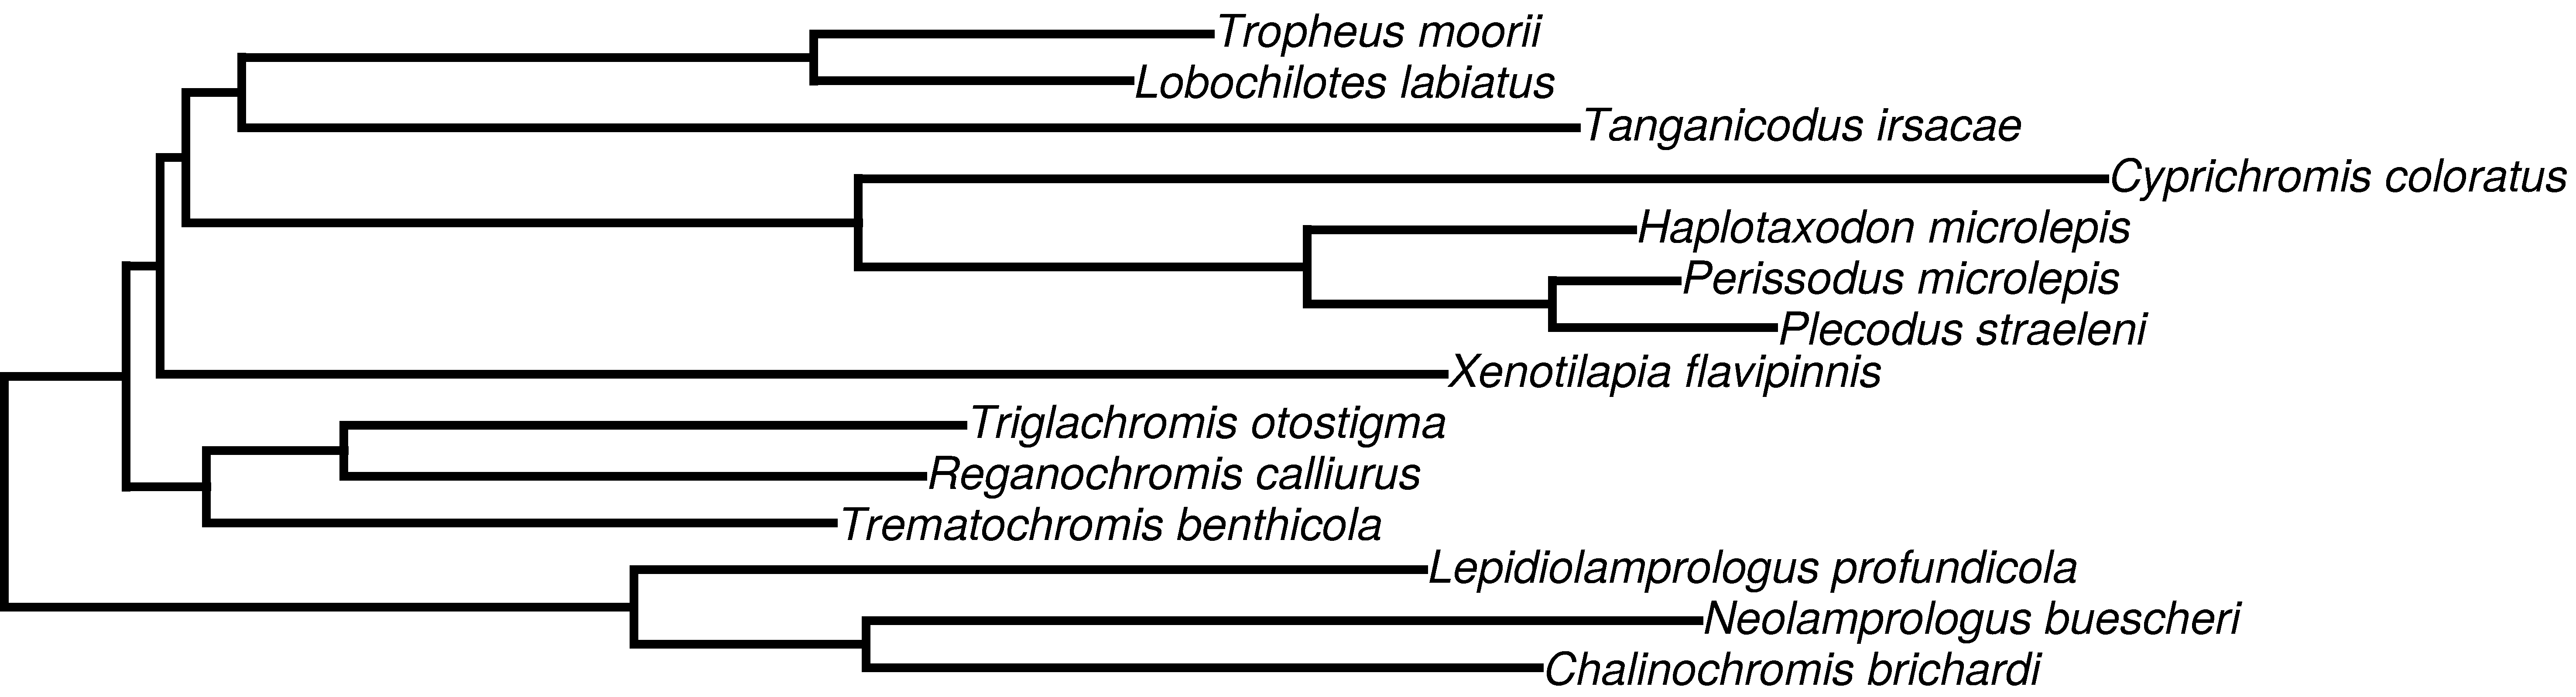
\includegraphics[width=\textwidth]{FishPoo/figures/mcgee_tree.pdf}
%    \caption{A maximum likelihood phylogeny of the host organisms.}
%    \label{FP_host_tree}
%\end{figure}

\subfile{FishPoo/figure2}

\subsection{Sample collection}

Specimens fed until satiated and placed into 30L tanks. To minimize microbial contamination in the water and tank silicone, we lined each tank with a sterile autoclave bag prepared with 10 liters of molecular water augmented with a small amount of sodium chloride and calcium chloride. To minimize potential contamination from biological filtration, we used chemical filtration via sterile charcoal pellets to sequester nitrogenous wastes produced by the fish, and a sterile plastic tube was submerged and connected to an air pump to aerate the water. Stool was removed using a sterile serological pipette and frozen. Fish remained in these tanks for less than 24 hours and were then returned to their original aquarium.

\subsection{Sample preparation, processing and sequencing}

Stool samples were subjected to bead beating for 60 seconds and DNA was extracted using MoBio PowerSoil DNA Isolation kit. 16S PCR and Illumina sequencing was carried out using the Earth Microbiome 16S Illumina Amplicon Protocol. 

\subsection{Building the observation table}

Adapter removal, quality trimming and overlap alignment is performed using {\tt Trimmomatic}. \cite{bolger2014trimmomatic} Chimera are identified with {\tt vsearch}, \cite{rognes2016vsearch} and unique reads are identified using {\tt hat-trie}. \cite{askitis2005cache, askitis2007hat} A table of observation counts is constructed as a {\tt Pandas} {\tt DataFrame} object, \cite{mckinney2010data} and a count threshold is applied. Tables of raw counts and normalized counts are written as comma separated value files, and the corresponding sequences are written as a FASTA file. All analysis was carried out and documented in Jupyter Notebooks \cite{perez2007ipython} and visualizations, including all those appearing in this manuscript, were constructed using {\tt Matplotlib}. \cite{hunter2007matplotlib}

\subsection{Building phylogeny of OTUs}

Alignment of the observed sequences is performed using {\tt Clustal Omega}, \cite{goujon2010new, sievers2011fast} and an approximate maximum likelihood phylogeny is constructed using {\tt FastTree}. \cite{price2009fasttree, price2010fasttree}

%\begin{figure}
%    \includegraphics[width=\textwidth]{FishPoo/figures/fishpoo_tree.png}
%    \caption{An approximate maximum likelihood phylogeny of the guest organisms.}
%    \label{FP_guest_tree}
%\end{figure}

\subfile{FishPoo/figure3}

\subsection{Spectral analysis and machine learning}

The host tree and guest tree are loaded as {\tt SuchTree} objects, and linked together through the observation table as a {\tt SuchLinkedTrees} object. The {\tt SuchTree} class allows for extremely rapid traversals of large trees, enabling distance correlations to be efficiently computed. The {\tt SuchLinkedTrees} class leverages this to compute graph adjacency and graph Laplacian matrixes of subtrees of host and guest phylogenies. Spectral decomposition and kernel densities of graph Laplacians are computed using {\tt numpy}, and the Jensen-Shannon divergence is calculated between each pair of spectral densities using the {\tt entropy} function in {\tt scipy.stats}. \cite{walt2011numpy} Feature tables were assembled using {\tt Pandas} \cite{mckinney2010data} and machine learning was carried out using {\tt scikit-learn}. \cite{pedregosa2011scikit}

\subsection{Correlation-based analysis}

For each clade of guest organisms, the {\tt SuchLinkedTrees.linked\_distances} function is used to calculate the pairwise distances through the host and guest trees for every pair of non-null observations in the link matrix, as described by Hommola {\em et al.} \cite{hommola2009permutation} The Pierson's correlation for these distances is computed using the {\tt pearsonr} function from {\tt scipy.stats}. \cite{walt2011numpy}

\subsection{Literature search for comparative analysis}

Trees and interaction matrixes were compiled from the supplementary material from Rezende {\em et al.}, \cite{rezende2007non} Hafner {\em et al.} \cite{hafner1994disparate} and Escudero \cite{escudero2015phylogenetic} for a total of fifty data sets (Table \ref{FP_studies_table}). Synthetic interactions with perfect phylogenetic congruence and with no phylogenetic congruence were simulated using {\tt Dendropy}. \cite{sukumaran2010dendropy} NEEDS DETAIL ON SIMULATIONS